\subsection*{\lr{2.6.1} تجزیهٔ فرمول‌ها به مجموعه‌ای از لفظ‌ها}
  \begin{definition}[تعریف \lr{2.57}]
    یک \emph{لفظ} (literal)، یا \emph{اتم} است یا \emph{نفی یک اتم}.
    \begin{itemize}
      \item یک اتم، \emph{لفظِ مثبت} نامیده می‌شود.
      \item نفی یک اتم، \emph{لفظِ منفی} نام دارد.
    \end{itemize}
    برای هر اتم $p$، مجموعهٔ $\{p,\;\neg p\}$ یک \emph{زوج متمم} از لفظ‌ها تشکیل می‌دهد.  
    برای هر فرمول $A$، مجموعهٔ $\{A,\;\neg A\}$ نیز یک \emph{زوج متمم از فرمول‌ها} است.  
    فرمول $A$ متمم $\neg A$ و بالعکس است.
  \end{definition}
    
  \begin{example}[مثال \lr{2.58}]
    در مجموعهٔ لفظ‌ها
    \[
    \{\neg p,\; q,\; r,\; \neg r\}
    \]
    \begin{itemize}
      \item $q$ و $r$ لفظِ \emph{مثبت} هستند،
      \item $\neg p$ و $\neg r$ لفظِ \emph{منفی} هستند.
    \end{itemize}
    این مجموعه شامل زوج متمم $\{r,\neg r\}$ است.
  \end{example}
    
  \begin{example}[مثال \lr{2.59}]
    فرمول زیر را تحلیل می‌کنیم تا ارضاپذیری آن را در تعبیر دلخواه $\mathscr{I}$ بررسی کنیم:
    \[
    A = p \land (\neg q \lor \neg p).
    \]
    با استفاده از قواعد بازگشتی ارزیابی صدق:
    \begin{align*}
    v_{\mathscr{I}}(A)=T
    &\;\Longleftrightarrow\;
    v_{\mathscr{I}}(p)=T
    \;\land\;
    v_{\mathscr{I}}(\neg q\lor\neg p)=T,\\
    v_{\mathscr{I}}(\neg q\lor\neg p)=T
    &\;\Longleftrightarrow\;
    v_{\mathscr{I}}(\neg q)=T
    \;\lor\;
    v_{\mathscr{I}}(\neg p)=T.
    \end{align*}
    در نتیجه، $v_{\mathscr{I}}(A)=T$ اگر و تنها اگر یکی از دو حالت زیر برقرار باشد:
    \begin{enumerate}
      \item $v_{\mathscr{I}}(p)=T$ و $v_{\mathscr{I}}(\neg q)=T$
      \item $v_{\mathscr{I}}(p)=T$ و $v_{\mathscr{I}}(\neg p)=T$
    \end{enumerate}
    پس مسئلهٔ ارضاپذیری $A$ به بررسی ارضاپذیری دو مجموعهٔ لفظ‌ها کاهش می‌یابد.
  \end{example}
    
  \begin{theorem}[قضیه \lr{2.60}]
    مجموعه‌ای از لفظ‌ها \emph{ارضاپذیر} است \emph{اگر و تنها اگر} شامل هیچ \emph{زوج متممی} از لفظ‌ها نباشد.
  \end{theorem}
    
  \begin{proof}
    فرض کنید $L$ مجموعه‌ای از لفظ‌ها باشد که هیچ زوج متممی در آن وجود ندارد. تعبیر $\mathscr{I}$ را به‌صورت زیر تعریف می‌کنیم:
    \[
    \mathscr{I}(p)=
    \begin{cases}
    T, & \text{اگر  } p\in L,\\
    F, & \text{اگر  } \neg p\in L.
    \end{cases}
    \]
    این تعریف \emph{سازگار و کامل} است، زیرا در $L$ هیچ اتمی همراه نقیضش حضور ندارد. هر لفظِ موجود در $L$ در این تعبیر مقدار $T$ می‌گیرد؛ بنابراین $L$ ارضاپذیر است.
    
    حال اگر $\{p,\neg p\}\subseteq L$، در هر تعبیر ممکن یا $v_{\mathscr{I}}(p)=F$ یا $v_{\mathscr{I}}(\neg p)=F$ است، پس $L$ ارضاپذیر نخواهد بود.
  \end{proof}
    
  \begin{example}[مثال \lr{2.61}]
    ادامهٔ مثال \lr{2.59}:  
    برای $A = p\land(\neg q\lor\neg p)$، دو مجموعه‌ای که باید بررسی شوند:
    \[
    \{p,\neg p\}\quad\longrightarrow\quad\text{دارای زوج متمم}\;\to\;\text{ناتوان از ارضا},
    \]
    \[
    \{p,\neg q\}\quad\longrightarrow\quad\text{فاقد زوج متمم}\;\to\;\text{ارضاپذیر}.
    \]
    بنابراین فقط مجموعهٔ دوم ارضاپذیر است و از قضیهٔ \lr{2.60} تعبیری به‌دست می‌آید که در آن
    \[
    \mathscr{I}(p)=T,\quad \mathscr{I}(q)=F.
    \]
  \end{example}
    
  \begin{example}[مثال \lr{2.62}]
    اگر فرمول \emph{ناتوان از ارضا} باشد، مثلاً:
    \[
    B = (p\lor q)\land(\neg p\land\neg q),
    \]
    آنگاه:
    \begin{enumerate}
      \item برای ارضا شدن $B$ باید
        $v_{\mathscr{I}}(p\lor q)=T$ و $v_{\mathscr{I}}(\neg p\land\neg q)=T$.
      \item تجزیهٔ ترکیب عطفی و ترکیب فصلی نشان می‌دهد که دو حالت ممکن به مجموعه‌های لفظ‌ها می‌انجامد:
        \[
        \{p,\neg p,\neg q\},\quad \{q,\neg p,\neg q\}.
        \]
      \item هر دو شامل زوج متمم‌اند؛ بنابراین ناتوان از ارضا هستند (قضیهٔ \lr{2.60}).
    \end{enumerate}
    نتیجه می‌گیریم که \emph{هیچ مدلی برای $B$ وجود ندارد}، یعنی
    \[
   \text{ناتوان از ارضا است.} B\
    \]
  \end{example}
  
  \begin{figure}[ht]
    \centering
    \begin{latin}
      \resizebox{0.35\textwidth}{!}{
      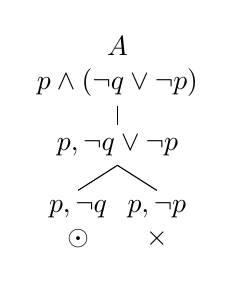
\begin{tikzpicture}[
        level distance=1cm,
        sibling distance=1.5cm,
        level 2/.style={sibling distance=1cm},
        edge from parent path={(\tikzparentnode.south) -- (\tikzchildnode.north)}
      ]
      \node[align=center] {$A$ \\ $p \land (\neg q \lor \neg p)$}
        child { 
          node {$p, \neg q \lor \neg p$}
          child { node[align=center] {$p, \neg q$ \\ $\odot$} }
          child { node[align=center] {$p, \neg p$ \\ $\times$} }
        };
      \end{tikzpicture}
      }
    \hfill
    \resizebox{0.35\textwidth}{!}{
      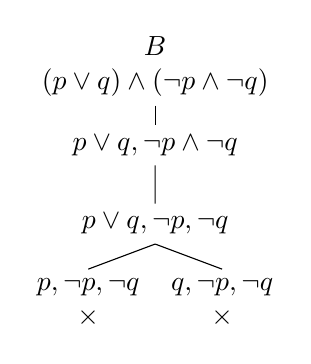
\begin{tikzpicture}[
        level distance=1cm,
        sibling distance=1.5cm,
        level 2/.style={sibling distance=1cm},
        level 3/.style={sibling distance=1.7cm},
        edge from parent path={(\tikzparentnode.south) -- (\tikzchildnode.north)}
      ]
      \node[align=center] {$B$ \\ $(p \lor q) \land (\neg p \land \neg q)$}
        child { 
          node {$p \lor q, \neg p \land \neg q$}
          child {
            node {$p \lor q, \neg p, \neg q$}
            child { node[align=center] {$p, \neg p, \neg q$ \\ $\times$} }
            child { node[align=center] {$q, \neg p, \neg q$ \\ $\times$} }
          }
        };
      \end{tikzpicture}
      }
    \end{latin}
    \renewcommand{\thefigure}{\lr{2.7}}
    \caption{درخت صدق}
  \end{figure}